\documentclass[german,oneside,color]{htldipl}
\usepackage{blindtext}
\usepackage[T1]{fontenc}
\usepackage[utf8]{inputenc}
\usepackage{array}
\usepackage{biblatex}
\usepackage{footmisc}

\graphicspath{{images/}}    % Bilderverzeichnis
\usepackage[paper=a4paper,margin=3cm]{geometry}

\makeindex[title=Index]
\makeindex[name=allgemein, title=Allgemeiner Index]
\makeindex[name=name,title={Autoren Index}]
\makeindex[name=title,columns=1,title={Literatur Index}]
\indexsetup{level=\subsection*, toclevel=subsection, noclearpage}


\makeatletter
\@ifpackageloaded{biblatex_legacy}
  {\DeclareIndexNameFormat{default}{%
     \usebibmacro{index:name}{\index[name]}{#1}{#3}{#5}{#7}}}
  {\DeclareIndexNameFormat{default}{%
     \usebibmacro{index:name}{\index[name]}
       {\namepartfamily}
       {\namepartgiven}
       {\namepartprefix}
       {\namepartsuffix}}}
\makeatother

\DeclareIndexFieldFormat{indextitle}{%
  \usebibmacro{index:title}{\index[title]}{#1}}

\renewbibmacro*{bibindex}{%
  \ifbibindex
    {\indexnames{author}%
     \indexnames{editor}%
     \indexnames{translator}%
     \indexnames{commentator}%
     \indexfield{indextitle}}
    {}}

\makeatletter
\DeclareCiteCommand{\repeatfootcite}[\cbx@wrap]
  {\gdef\cbx@keys{}}
  {\xappto\cbx@keys{\thefield{entrykey},}}
  {}
  {\ifcsundef{cbx@lastin@\cbx@keys @\strfield{postnote}}
     {\csnumgdef{cbx@lastin@\cbx@keys @\strfield{postnote}}{-1}}{}%
   \ifsamepage{\value{instcount}}{\csuse{cbx@lastin@\cbx@keys @\strfield{postnote}}}
     {\footnotemark[\csuse{cbx@lastfn@\cbx@keys @\strfield{postnote}}]}
     {\xappto\cbx@cite{\noexpand\footcite%
        [\thefield{prenote}][\thefield{postnote}]{\cbx@keys}%
        \csnumgdef{cbx@lastfn@\cbx@keys @\strfield{postnote}}{\value{\@mpfn}}%
        \csnumgdef{cbx@lastin@\cbx@keys @\strfield{postnote}}{\value{instcount}}}}}

\newrobustcmd{\cbx@wrap}[1]{#1\cbx@cite\gdef\cbx@cite{}}
\def\cbx@cite{}
\makeatother
\addbibresource{literatur.bib}
 
 \newcommand{\putz}
 {\marginpar{\scriptsize{\textit{$\rightarrow$Putz}}}}
 
  \newcommand{\strahlhofer}
 {\marginpar{\scriptsize{\textit{$\rightarrow$Strahlhofer}}}}
 
  \newcommand{\bauer}
 {\marginpar{\scriptsize{\textit{$\rightarrow$Bauer}}}}
 
  \newcommand{\reiter}
 {\marginpar{\scriptsize{\textit{$\rightarrow$Reiter}}}}

\begin{document}

\title{EMS - Event Management Software zum Verwalten und Organisieren von Events jeglicher Art und deren Werbetreibender}
\abteilung{Informatik}
\schwerpunkt{Ausbildungsschwerpunkt Informatik}
\studienort{Wiener Neustadt}
\schule{HTBLuVA Wiener Neustadt}
\schullogo{htl.jpeg}
\abgabejahr{2020/21}
\betreuerA{Dipl.-Ing. Harald Breidler}
\betreuerB{}
\betreuerC{}
\schuelerA{Maurice PUTZ}
\evidenzA{5AHIF-16}
\subthemaA{Grundlagen der DSGVO mit Schwerpunkt auf Datenschutzfreundlicher Entwicklung von Software und Nutzung von Cloud Computing}
\schuelerB{Benjamin STRAHLHOFER}
\evidenzB{5AHIF-20}
\subthemaB{Benjamin Strahlhofer - Subthema}
\schuelerC{Thomas BAUER}
\evidenzC{5AHIF-2}
\subthemaC{Thomas Bauer - Subthema}
\schuelerD{Alexander REITTIER}
\evidenzD{5AHIF-KA}
\subthemaD{Alexander Reiter - Subthema}
\schuelerE{}
\evidenzE{}
\subthemaE{}

%%%----------------------------------------------------------
\frontmatter
\maketitle
\tableofcontents
\listoffigures

%%%----------------------------------------------------------

%Hier kommen die Includes für die Einleitung	
%\chapter{Vorwort}
Dieses Dokument wurde im Rahmen der Reife- und Diplomprüfung 2020/21 an der Höheren Technischen Bundes-, Lehr- und Versuchsanstalt Wiener Neustadt verfasst. Die Idee für dieses Projekt ging von vier engagierten HTL Schülern aus, durch
private Erfahrungen im Management, Marketing und der Organisation betreffend Events und Veranstaltungen. Daraufhin entstand die Idee, mithilfe einer Software viel manuellen Aufwand in der Organisation von Events zu automatisieren. Zuerst zusammen mit einem Unternehmen
welches seine Tätigkeit als Event planer ausführt, wurde die Idee letztendlich von uns vier weiter ausgebaut und realisiert.
Die Software ist bei Release eine individuelle Anwendung, welche später, durch verschiedene Upgrades im allgemeinen lizenziert vergeben werden soll.\newline
Eine maßgeblich daran beteiligte Person und auch Initiator des Unterfangens, konnte die Idee leider nicht mit uns in der Projektgruppe aufgrund gewisse Komplikationen, umsetzen.\newline
Vielen Dank an Herrn Peter Hammer, für seine Ideen und maßgeblich Entscheidende Anfangsidee für so ein Projekt.
Besonderer Dank gilt unserem äußerst engagierten Betreuer, Herrn Prof. Harald Breidler, dass er zu Jahresanfang freiwillig unsere Projektgruppe noch im letzten Moment betreute. Weiters Danken wir herzlich unserem SYP-Lehrer, Herr Prof. Markus Reis
welcher uns im Laufe dieses Projekts jederzeit mit einem gutem Rat zur Seite stand. 
Des Weiteren gilt unseren Familien und Freunden besonderer Dank, die uns in dieser stressigen Zeit viel Kraft gegeben haben. 

%%Inkludiert die 4. vorgeschriebenen Seiten an Dokumentation aus dem gedruckten PDF-Formular
%Das Formular erst vor der Abgabe vollständig ausfüllen, da z.B. das Bild zur Diplomarbeit vorher nicht vorhanden sein wird
\begingroup
\makeatletter
\newpage
\@twosidefalse
\includepdf[pages=1-1,pagecommand={\chapter[Diplomarbeit Dokumentation]{}}]{pdf/Formular-printed.pdf}
\includepdf[pages=2-2,pagecommand={\thispagestyle{plain}}]{pdf/Formular-printed.pdf}
\includepdf[pages=3-3,pagecommand={\chapter[Diploma Thesis Documentation]{}}]{pdf/Formular-printed.pdf}
\includepdf[pages=4-4,pagecommand={\thispagestyle{plain}}]{pdf/Formular-printed.pdf}
\endgroup

%\chapter{Kurzfassung}
Die Software EMS soll in jeder Situation ein professionelles Eventmangement ermöglichen.
Die Kernaufgaben liegen darin, dass Benutzer und Tickets zusammen mit Events verwaltet werden können.
Sogenannte Influencer und Promoter, welche hauptsächlich Personen mit einer großen Reichweite auf Social Media Kanälen sind, ist die neueste Art von Marketing und verspricht für ein Event schnell, viel Aufmerksamkeit zu bekommen.
Diese App soll eine Plattform bieten, diese Influencer und Promoter leicht und überschaulich zu verwalten und das Marketing eines Event dadurch besser zu koordinieren.
Weiters soll durch die Applikation der Eintrittsticketverkauf und der Prozess dahinter, vor allem organisatorisch verbessert und übersichtlicher gemacht werden. 
Die Software unterscheidet einen Benutzer anhand von zwei Rollen, eine Rolle ist die des Promoters, die andere ist die eines Administrators.

Die Anwendung gliedert sich in drei verschiedene Hauptseiten auf, wovon zwei einem normalen Promoter zugänglich sind.
Jeder Promoter hat ein Profil mit seinem Namen, einem Profilbild und einer Beschreibung. Dieses Profil können die Promoter selbst anpassen. Der Name ist jedoch nicht von einem normalen Promoter änderbar.
Die Hauptseite umfasst die Übersicht aller Events. Hier werden alle dem Promoter zugeteilten Events, für welche er Karten verkaufen soll, angezeigt.
Er kann auf eines der Events klicken und gelangt dadurch auf eine detailliertere Seite der gewählten Veranstaltung.
Hier kann er seinen Kartenstand aktualisieren. Für jede verkaufte Karte oder jedes verkaufte Package (Sammlung von Karte) bekommt ein Promoter sogennante Goodie-Punkte.
Diese Punkte kann er dann auf der Event-Details Seite für bestimmte Goodies eintauschen, wie beispielweise \textbf{Ein gratis Getränk beim Event für 10 Punkte}.

Die letzte Seite ist das Admin-Terminal. Wie der Name schon sagt steht diese Seite nur einem Administrator zur Verfügung.
Hier kann dieser einen Benutzer erstellen, ihn deaktivieren und aktivieren und einem Benutzer einem Event zuweißen.
Weiters werden hier auch die Events erstellt indem man Kartentypen, Packages und Belohnungen für die Goodie-Punkte zum einlösen, festlegt.

\textbf{Hinweis:} Sämtliche angegebenen Quellen und Links wurden mit Stand 20.04.2021, 16:00 auf Ihre Richtigkeit und Integrität überprüft.
Sie entsprechen dem momentanen Stand des Wissens in ihren jeweiligen Gebieten zu gegebenem Datum.
Änderungen der Quellen nach angegebenem Zeitpunkt wurden nicht in dieses Dokument übernommen.
Falls solche stattfinden ist das Dokument als veraltet zu betrachten und muss aktualisiert werden.
Die Daten bei den Quellen wurden mithilfe eines selbst erstellten JavaScripts auf ihre aktualität überprüft.
%\include{Abstract}

%%%----------------------------------------------------------
\mainmatter           %Hauptteil (ab hier arab. Seitenzahlen)
%%%----------------------------------------------------------
%\appendix
%Hier kommen die Includes für den Hauptteil
%\chapter{Einleitung}
\section{Ausgangslage}
Bei Veranstaltungen mit einer Alterszielgruppe von 16-21 - jährigen wird heutzutage oft auf Marketing mit Influencer und Promoter gesetzt. 
Sogenannte Influencer und Promoter sind hauptsächlich auf Instagram, Facebook und anderen Social-Media Netzwerken tätig und bewerben dort das jeweilige Event. 
Nachdem eine Nachfrage nach Eintrittskarten besteht, ist es die Aufgabe der Promoter den Eintrittskartenvertrieb zu übernehmen. 
Influencer bewerben weiterhin nur das Event und verkaufen allerdings keine Karten. 
Bei diesen Events müssen 100-150 Promoter Karten erhalten, verkaufen und zu einen späteren Zeitpunkt das eingenommen Geld abgegeben. Dadurch entsteht eine großer 
administrativer Aufwand. Aktuell wird alles mit Hand geführten Protokollen und Listen dokumentiert. Dies sorgt bei dieser Anzahl an Daten schnell für Fehler desen suche
oft viel Zeit in Anspruch nimmt. Für die Auswertung der gesammelten Daten wird eine hochkomplexe Excel Liste benutzt. Leider ist dieser Prozes oft ungenau und wichtige 
Daten gehen verloren oder der Verlauf ist später nicht mehr nachvollziehbar. 

\section{Ziele}
Durch eine iOS und Android App soll den Promoter-Managern und der Eventleitung viel organistorischer Aufwand abgenommen werden. Weiters soll die Fehlerquote stark gesenkt werden
wodurch in manchen Fällen viel Geld gespart werden kann. 

\newpage
\section{Team}
\subsection{Maurice Putz}
\subsubsection{Themenstellung}
Chatsystem in EMS, Cloud Computing und Beispiel eines Backend Deployment in AWS mit Schwerpunkt auf Grundlagen im Datenschutz und DSGVO Konformität
\subsubsection{Rolle}
In diesem Projekt übernahm er die Rolle eines Fullstack Entwickler. Er hatte die Verantwortung für das Chatsystem,
sowie zahlreiche Funktionen im Front- sowie Backend. Außerdem war er für das Deployment des Backend der App am Ende zuständig.

\subsection{Benjamin Strahlhofer}
\subsubsection{Themenstellung}
Anmeldesystem in EMS, Sicherheitsrisiken Abwicklung und Vergleich ein Biometrie, mit dem Schwerpunkt auf Sicherheit eines Anmeldesystems
\subsubsection{Rolle}
In diesem Projekt Übernahm er die Rolle eines Fullstack Entwickler. Er hatte die Verantwortung für das Anmeldesystem und 
sowie zahlreiche Funktionen im Front- und Backend.

\subsection{Thomas Bauer}
\subsubsection{Themenstellung}
Allgemeines zu Data Analytics und Grundlagen von Rest API's, Vergleich von SQL und einer NoSQL Datenbank mit Schwerpunkt auf Datenbankentwurf
\subsubsection{Rolle}
In diesem Projekt Übernahm er die Rolle eines Fullstack Entwickler. Er hatte die Verantwortung über die Datenbank, 
sowie zahlreiche Funktionen im Front- und Backend. 

\subsection{Alexander Reiter}
\subsubsection{Themenstellung}
Ticketsysteme, Untersuchung von Belohnungssystemen für Wettbewerbssituationen und Vorgehensmodelle mit Schwerpunkt auf einem Vergleich von SCRUM und RUP
\subsubsection{Rolle}
JA WAS DENN? HA HA HA? GOR NIX, KONNST NIX, SCHENE GRIAS

\newpage

%ZB
\chapter{Grundlagen von Cloud Computing}
\putz

%Quellen: Reisi Folien, %Quellen: Reis Folien, https://de.wikipedia.org/wiki/Cloud_Computing#Servicemodelle

\section{Cloud Computing Definition}
\subsection{Allgemeines}
Es gibt einige verschiedene Definition des Begriffs Cloud Computing, einer sehr präzise Beschreibung wäre:

\begin{center}
   \textit{Ein Modell zur Bereitstellung von einer Reihe von Services für Unternehmen oder anderweitige Konsumenten über das Internet, wie zum Beispiel das
	Speichern von bestimmten Daten oder das Hosten einer Webseite auf einem Webserver. Die Services sind nicht nur auf Software Angebote beschränkt, es kann zum Beispiel auch Rechenleistung
	angeboten werden. Der Service läuft aus der Sicht des Konsumenten extern beim Anbieter der Services, dem sogenannten Provider.}
\end{center}

Jede Cloud hat bestimmte Eigenschaften welche den Begriff definieren, diese teilen sich in drei Hauptbereiche aus:
\begin{itemize}
	\item die zentralen, essenziellen Charakteristiken einer Cloud
	\item Servicemodelle
	\item Deployment Models oder Bereitstellungsmodelle
\end{itemize}

%Quellen: Reis Folien, https://de.wikipedia.org/wiki/Cloud_Computing

\subsection{Charakteristiken einer Cloud}
Jede Cloud hat bestimmte spezielle Charakteristiken, das NIST \textbf{(National Institute of Standard and Technology)} listet
momentan fünf essenzielle Eigenschaften die da wären:
\begin{itemize}
	\item \textbf{On-demand self-service: } Bedeutet, dass Ressourcen wie etwa Speicher und Rechenleistung der Cloud, vom Nutzer selbstständig oder automatisiert 
ohne persöhnliche Interaktion mit dem Service Provider in Anpsruch genommen werden kann
	\item \textbf{Broad network access: } Services aus der Cloud sind über das Internet und durch Standardmechanismen, mithilfe von verschiedenen Plattformen
wie einem Smartphone, einem Laptop, einem Stand-PC oder Tablet, erreichbar
	\item \textbf{Resource pooling: } Die in generell in einer Cloud zu Verfügung stehenden Ressourcen wie zum Beispiel Speicher und Rechenleistung sind für alle Kunden gebündelt von einem Pool aus verfügbar und werden geteilt, dabei ist der physische Standort der Server für den Klienten in der Regel unbekannt.
	\item \textbf{Rapid elasticity: } Die durch den Kunden in Anspruch genommenen Ressourcen können aus dessen Sicht, schnell ins beinahe unendliche skaliert werden, die Lastenänderung
kann ebenfalls automatisiert angepasst werden, sodass keine menschliche Interaktion notwendig ist.
	\item \textbf{Measured Service: } Die Ressourcennutzung der Kunden kann durch den Anbieter gemessen, überwacht und analysiert werden, zum Zwecke von Abrechnungen, einer effektiver
Nutzung der in Anspruch genommenen Ressourcen oder für eine vorausschauende Gesamtplanung.
\end{itemize}

%Quellen: Reis Folien, https://de.wikipedia.org/wiki/Cloud_Computing#Servicemodelle,
%https://azure.microsoft.com/de-de/overview/what-is-cloud-computing/#cloud-computing-models

\subsection{Servicemodelle}
NIST listet drei grundsätzliche Standard-Modelle, in welcher Form Cloud-Computing Dienste angeboten werden können, diese werden oft als Schichten untereinander vereinfacht dargestellt:
\begin{itemize}
	\item Infrastructure as a Service (IaaS)
	\item Platform as a Service (PaaS)
	\item Software as a Service (Saas)
\end{itemize}


Zusätzlich zu den oben genannten standardisierten Modellen, existieren noch einige weitere Modelle auf dem Markt. Prinzipiell
kann man heutzutage fast jeden nur denkbaren Service über eine Cloud beziehen, mit der Zeit haben sich dafür spezielle Bezeichnungen gebildet. Diese Fachbegriffe können zusammengefasst werden:
\begin{itemize}
	\item Function as a Service (FaaS) oder Serverless computing
	\item Everything as a Service (XaaS)

\end{itemize}

%Quellen: Reis Folien, https://de.wikipedia.org/wiki/Cloud_Computing#Servicemodelle,
%https://azure.microsoft.com/de-de/overview/what-is-cloud-computing/#cloud-computing-models,
%https://de.wikipedia.org/wiki/Everything_as_a_Service#Infrastructure_as_a_Service_(IaaS),

\subsubsection{Infrastructure as  a Service (IaaS)}
Bei IaaS nimmt der Kunde IT-Infrastruktur wie Server, Speicher und Virtuelle Computer von einem Cloudanbieter in Anspruch. In diesem Fall gestaltet der Kunde seine eigene Infrastruktur selbst innerhalb einer Cloud und kümmert sich um die Installation von Software und den laufenden Betrieb derer selbst. Der Anbieter ist lediglich für die genutzten physischen Hardware Elemente verantwortlich und wartet diese, alles andere fällt in den Zuständigkeitsbereich des Kunden. Kurz zusammengefasst ist IaaS Bereitstellung von Infrastruktur über das Internet, welche vom Nutzer bedingt kontrolliert wird. \newline
Infrastructure as a Service kann auch als Everything as a Service bezeichnet werden, da in diesem Geschäftsmodell alles vom Kunden selbst verwaltet wird. Einige Charakteristiken von IaaS:
\begin{itemize}
	\item Nur einmalig genutzte Anwendungen werden einmal bezahlt und wieder freigegeben
	\item Im Falle eines explosionsartigen Wachstums und ein erreichen der Belastungsspitzen kann abgefangen werden, da die Services in jede Richtung skalierbar sind. So können innerhalb von Minuten zum Beispiel viel Speicher erweitert werden oder auch im Gegenteil nicht genutzte Kapazitäten frei gegeben werden, welche dann nicht mehr bezahlt werden müssen.
\end{itemize}

Ein Beispiel dafür wäre das Mieten eines VPS-Servers (Virtual Private Server) um eine Webapp wie EMS darauf aufzusetzen.
Als Kunde mietet man eine gewisse Größe an Hauptspeicher (RAM) und Nebenspeicher (SSD), eine Anzahl an CPU-Kernen, wie groß die Bandbreite seien soll und noch viele andere Optionen, welche bei jedem Cloudanbieter variieren. Auf diesem VPS-Server kann man nun sein Front- und Backend aufsetzen und hat über alles selbst die Kontrolle. Klassische Anbieter welche IaaS anbieten wären Amazon mit Amazon Web Services (AWS) mit dem möglicherweise populärsten Service EC2.

%Quellen: Reis Folien, https://de.wikipedia.org/wiki/Cloud_Computing#Servicemodelle,
%https://azure.microsoft.com/de-de/overview/what-is-cloud-computing/#cloud-computing-models,
%https://de.wikipedia.org/wiki/Platform_as_a_Service

\subsubsection{Platform as a Service (PaaS)}
PaaS stellt dem Kunden eine Programmier- und Laufzeitumgebung zur Verfügung. Hier stellt der Cloudanbieter eine Softwareumgebung fertig aufgesetzt für den Nutzer zur Verfügung, damit dieser eigene Softwareanwendungen darauf entwickeln kann. Die Daten- und Rechenkapazitäten der Umgebungen sind dabei flexibel und können dynamisch hin Hinsicht auf Daten- und Rechenkapazität angepasst werden.\newline
\newline
Diese Form des Cloudservices würde sich vor allem an Unternehmen richten, welche eine große Anzahl an Mitarbeiter beschäftigt und an vielen Applikationen gleichzeitig arbeitet und diese schnell entwickeln muss, jedoch nicht genügend Kapital hat, um jeden Arbeitsplatz mit einer Rechenmaschine mit entsprechend benötigter Leistung auszurüsten. Stattdessen könnte solch eine Firma auf PaaS zurückgreifen und für einen geringen Betrag, monatlich diese Umgebungen in einer Cloud mieten und spart sich so viel Kapital und bleibt bei den benötigten Rechenleistungen flexibel, da die Umgebungen eben flexibel auf die benötigten Performanceansprüche skaliert werden kann. Dies wäre bei eingekaufter Hardware in einem Büro nicht so leicht, was dieses Servicemodell den Kunden auch schnell und einfach auf neue Technologien und Anforderungen reagieren lässt.

%Quellen: Reis Folien, https://de.wikipedia.org/wiki/Cloud_Computing#Servicemodelle,
%https://azure.microsoft.com/de-de/overview/what-is-cloud-computing/#cloud-computing-models,
%https://de.wikipedia.org/wiki/Software_as_a_Service

\subsubsection{Software as a Service (Saas)}
Manchmal auf als Software on Demand beschrieben, was "Software nach Bedarf" übersetzt bedeutet. Hier bietet der Cloudanbieter spezielle Software zur Nutzung an. Der Kunde kann dann diese Software- und Anwendungsprogramme nach belieben benutzen. Die Applikationen werden über das Internet dem Nutzer zur Verfügung gestellt, und dieser kann mittels einer API darauf zugreifen, was meistens über einen Browser oder eine App geschieht. Die Infrastruktur hinter den Anwendungen verwaltet der Anbieter selbst und auch die Angebotene Software könnte nur bis zu einem gewissen Teil vom Kunden konfiguriert werden. Also sämtliche Instandhaltungsarbeiten obliegen dem Cloudanbieter, der Nutzer benutzt lediglich die angebotene Software und kann sich bei Problemen nur an den Support wenden.\newline
\newline
Ein Beispiel für so einen Service wären die meisten Google Services wie Gmail, Docs, Drive und Photos. Noch weitere Prominente Beispiele für Software as a Service sind Github, Office 365 und Dropbox.

%Quellen: Reis Folien, https://de.wikipedia.org/wiki/Cloud_Computing#Servicemodelle,
%https://azure.microsoft.com/de-de/overview/what-is-cloud-computing/#cloud-computing-models,
%https://de.wikipedia.org/wiki/Function_as_a_Service

\subsubsection{Function as a Service (FaaS)}
Prinzipiell ist FaaS von den Angeboten und Leistungen ähnlich wie das vorhin beschriebene Paas-Modell. Es stellt eine Laufzeitumgebung zur Verfügung, worauf Softwareanwendungen erstellt werden könne. Der maßgebende Unterschied zwischen Function und Platform as a Service ist, dass bei PaaS die Skalierung mittels hinzufügen von weiteren Serverprozessen zu den bereits in Anspruch genommenen stattfindet. Dies bewirkt natürlich normalerweise eine Kostenerhöhung auf Seiten des Benutzers, welche direkt Abgebucht oder in Rechnung gestellt wird. Die Skalierung ist dem Benutzer hier dadurch aber auch sehr übersichtlich und man kann die Aus- und Belastung seiner Entwicklerumgebung leicht nachvollziehen.\newline
Ganz anders im Gegensatz dazu geschieht die Skalierung bei FaaS. Bei diesem Service läuft keine extra Serverinstanz im Hintergrund. Bei FaaS muss der Benutzer die \textbf{Function exceution time} bezahlen. Die Zeit zwischen den Ausführungen von Code wird hierbei nicht in Rechnung gestellt, also lediglich, wenn ein Code zum Beispiel Übersetzt wird oder ein Programm ausgeführt und getestet wird. Somit muss der Benutzer auch nicht mehr an die Skalierung denken, da seine Entwicklerumgebung quasi kostenlos zu Verfügung steht und er nur die Ausführung der Software nach deren Zeitaufwand bezahlen muss. Dies sorgt für geringere Kosten auf Seiten des Kunden, bei gleichzeitig höhere Skalierbarkeit, da diese nicht mehr beachtet werden muss. Einen Nachteil gibt es jedoch und zwar kann die Latenz bei diesem Server höher als bei einer Lösung mit PaaS sein. Dies ist jedoch von vielen Faktoren und nicht zuletzt auch von der Komplexität des kodierten Programmes abhängig.

Dieser Service verfolgt den Ansatz des sogenannten \textbf{"serverless computing"}. Hierbei übernimmt der Cloud-Anbieter die komplette Ressourcenzuweisung, zum Beispiel benötigter Speicher und benötigte Prozessorkernanzahl, für den Kunden. Bei serverless computing wird keine Ressource im volatilen Speicher gehalten. Dies bedeutet, Berechnungen werden in bestimmten Abständen durch bestimmte Events von Seiten des Kunden aus, ausgelöst und die Ergebnisse werden dann in einen persistenten Speicher geschrieben. Wenn eine Anwendung gerade nicht vom Kunden benutzt wird, wird dies auch nicht in Rechnung gestellt wie es bei herkömmlichen Services der Fall ist. Es gibt keinen fixierten Betrag der monatlich oder Quartals mäßig abgebucht wird, sondern nur produktiv genutzte Zeit in der Anwendung wird berechnet.

Das erste offizielle, kommerzielle Angebot eines solchen Services gab es 2006. Seitdem haben viele große Cloud-Anbieter wie zum Beispiel Amazon mit AWS Lambda, Google und Microsoft mit Azure, solche \textbf{pay as you go} Services zu Verfügung gestellt.

\subsubsection{Everything as a Service (XaaS)}



\newpage
 
\chapter{Datenschutzgrundverordnung (DSGVO)}
\putz

%Quellen:
%Reis Folien
%https://de.wikipedia.org/wiki/Datenschutz-Grundverordnung
%https://wirtschaftslexikon.gabler.de/definition/datenschutz-grundverordnung-99476
\section{Aufbau und Inhalt}
\subsection{DSGVO Grundsätze}
Die Datenschutzgrundverordnung, oder im englischen Sprachraum \textbf{General Data Protection Regulation (GDPR)} genannt, soll die Rechte von natürlichen, realen Personen im Bezug auf Verarbeitung deren personenbezogenen Daten, genau definieren und sicherstellen. Die DSGVO wurde am 25. Mai 2016 beschlossen und trat in Kraft. Sie musste ab diesem Zeitpunkt unter Einhaltung einer zwei jährigen Umsetzungsfrist bis 25. Mai 2018 eingehalten werden. Primär soll jedem EU-Bürger das Recht auf informelle Selbstbestimmung garantiert werden und jeder Mensch in der EU soll vor nicht sachgerechter Nutzung der eigenen Daten rechtlich geschützt werden.
Die neue Datenschutz Richtlinie der Europäischen Union ersetzt die bis dahin geltenden \textbf{Datenschutzrichtlinie 95/94}. Das Gesetz wurde als EU Verordnung erlassen und somit in allen Mitgliedsstaaten vollständig übernommen werden. Die Verordnung enthält jedoch 69 sogenannte Öffnungsklauseln, welche den jeweilige Staate der Europäischen Union eine nationale Selbstbestimmung in diese Punkten erlaubt. Zum Beispiel das alter, ab welchem das Gesetz für eine Person gilt. Hier gilt ein Spielraum, dass das Alter, ab wann die DSGVO auf ein Individuum zutrifft, national selbstbestimmt werden kann, jedoch nicht über 16 und nicht unter 13 liegen darf.

Artikel 2, der sachliche Anwendungsbereich der DSGVO beinhaltet:
\begin{itemize}
	\item ganz oder teilweise automatisierte Verarbeitung von personenbezogener Daten
	\item manuelle Verarbeitung personenbezogener Daten, welche in einem Dateisystem gespeichert werden
\end{itemize}

Für die Verordnung gibt es gewisse Ausnahmen (Artikel 1, Abs. 2):
\begin{itemize}
	\item im Rahmen von Tätigkeiten, welche nicht in den Anwendungsbereich des Unionsrechts fallen
	\item Tätigkeiten im Rahmen der gemeinsamen Außen- und Sicherheitspolitik (Titel V, Kapitel 2 EUV)
	\item durch natürliche Personen zur Ausübung ausschließlich persönlicher oder familiärer Tätigkeiten
	\item durch die zuständigen Behörden zum Zwecke der Verhütung, Ermittlung, Aufdeckung oder Verfolgung von Straftaten oder der Strafvollstreckung, einschließlich des Schutzes vor und der Abwehr von Gefahren für die öffentliche Sicherheit
\end{itemize}

\subsection{Kapitel und Aufbau der DSGVO}
Die Datenschuttgrundverordnung ist in 11 Kapitel unterteilt. Diese Kapitel sind wiederum in einzelne Artikel unterteile, 99 an der Zahl. Eine Übersicht:

\begin{itemize}
	\item \textbf{Kapitel I (Artikel 1 bis 4)}: Allgemeine Bestimmungen
	\item \textbf{Kapitel II (Artikel 5 bis 11)}: Grundsätze und Rechtmäßigkeit
	\item \textbf{Kapitel III (Artikel 12 bis 23)}: Grundsätze und Rechtmäßigkeit
	\item \textbf{Kapitel IV (Artikel 24 bis 43)}: Verantwortlicher und Auftragsverarbeiter
	\item \textbf{Kapitel V (Artikel 44 bis 50)}: Übermittlungen personenbezogener Daten an Drittländer oder an internationale Organisationen
	\item \textbf{Kapitel VI (Artikel 51 bis 59)}: Unabhängige Aufsichtsbehörden
	\item \textbf{Kapitel VII (Artikel 60 bis 76)}: Zusammenarbeit und Kohärenz, Europäischer Datenschutzausschuss
	\item \textbf{Kapitel VIII (Artikel 77 bis 84)}: Rechtsbehelfe, Haftung und Sanktionen
	\item \textbf{Kapitel IX (Artikel 85 bis 91)}: Vorschriften für besondere Verarbeitungssituationen
	\item \textbf{Kapitel X (Artikel 92 bis 93)}: Delegierte Rechtsakte und Durchführungsrechtsakte
	\item \textbf{Kapitel XI (Artikel 94 bis 99)}: Schlussbestimmungen
\end{itemize}

\subsection{Definitionen}
Bestimmte Fachbegriffe wie "`natürliche Peron"' oder was sind personenbezogene Daten, sind in der EU Verordnung definiert und beschrieben worden.

\paragraph{}

%Quellen:
%https://www.privacypolicies.com/blog/privacy-by-design/
%https://gdpr-info.eu/issues/privacy-by-design/
%https://keyed.de/blog/software-dsgvo/#DSGVO%20Checkliste%20f%C3%BCr%20Software
\section{Capgemini studie 2019 und 2020}

\newpage

\chapter{Cloud Computing und AWS}
\putz

\section Bla
\section Bla Bla

\newpage
%\include{Vergleich_Putz}

%%%----------------------------------------------------------
%%%Anhang
%%%----------------------------------------------------------
%\appendix

%%Hier kommen die Includes für den Anhang

%%%----------------------------------------------------------
%Ausgabe der automatischen Zusatzdaten: Glossar, Index, Literaturverzeichnis
%\clearpage
%\printglossaries

\clearpage
\chapter*{Index}
\addcontentsline{toc}{chapter}{Index}
\printindex[allgemein]

\printindex

\printindex[name]

\printindex[title]


%Literaturverzeichnis
\clearpage
\addcontentsline{toc}{chapter}{\bibname}
\printbibliography

\clearpage
\chapter*{Messbox zur Druckkontrolle}



\begin{center}
{\Large --- Druckgröße kontrollieren! ---}

\bigskip

\Messbox{100}{50} % Angabe der Breite/Hoehe in mm

\bigskip

{\Large --- Diese Seite nach dem Druck entfernen! ---}

\end{center}



%%%----------------------------------------------------------
\end{document}